\documentclass{beamer}
\title{Intro to AI and ML}
\subtitle{Matrix Project}
\author{Christian Stavan Nilesh,
		\\Uttam Choudhary}

%\usetheme{lucid}
\begin{document}
	\frame {
		\titlepage
	}
	\frame {
		\frametitle{Geometry Question-}
		A circle passes through the points
		$\begin{pmatrix}
		2\\3
		\end{pmatrix}$
		and
		$\begin{pmatrix}
		4\\5
		\end{pmatrix}$. If its centre lies on the line
		\begin{equation}
		\begin{pmatrix}
		-1&4\\
		\end{pmatrix}\bold{x}+3=0
		\end{equation} find its radius.		
	}
	\frame{
		\frametitle{Solution-}
		Assume centre of required circle is given by $\bold{c}$ and radius $r$.
		Then equation of circle will be:
		\begin{equation}
		\bold{x}^T\bold{x}-2\bold{c}^T\bold{x}=r^2-\bold{c}^T\bold{c}
		\end{equation}
		Let $\bold{A}=\begin{pmatrix}
		2\\3
		\end{pmatrix}$ and $\bold{B}=\begin{pmatrix}
		4\\5
		\end{pmatrix}$ be the given points. Substituting the two points $\bold{A}$ and $\bold{B}$ in the equation of circle:
		\begin{equation}
		\begin{pmatrix}
		2&3\\
		\end{pmatrix}
		\begin{pmatrix}
		2\\3
		\end{pmatrix}-2\bold{c}^T\begin{pmatrix}
		2\\3
		\end{pmatrix}=r^2-\bold{c}^T\bold{c}
		\end{equation}
		and
		\begin{equation}
		\begin{pmatrix}
		4&5\\
		\end{pmatrix}
		\begin{pmatrix}
		4\\5
		\end{pmatrix}-2\bold{c}^T\begin{pmatrix}
		4\\5
		\end{pmatrix}=r^2-\bold{c}^T\bold{c}
		\end{equation}	
	}
	\frame{
		\frametitle{Solution(contd)-}
		On taking difference of above two equations ((4)-(3)) we get:
		\begin{equation}
		41-13-2\bold{c}^T\begin{pmatrix}
		2\\2
		\end{pmatrix}=0
		\end{equation}
		or
		\begin{equation}
		2\bold{c}^T\begin{pmatrix}
		2\\2
		\end{pmatrix}=28
		\end{equation}
		or
		\begin{equation}
		\bold{c}^T\begin{pmatrix}
		1\\1
		\end{pmatrix}=7
		\end{equation}
		on taking transpose both sides
		\begin{equation}
		\begin{pmatrix}
		1&1\\
		\end{pmatrix}\bold{c}=7
		\end{equation}
	}
	\frame{
		\frametitle{Solution(contd)-}
		It is also given that centre lies on line:
		\begin{equation}
		\begin{pmatrix}
		-1&4\\
		\end{pmatrix}\bold{x}=-3
		\end{equation}
		Using equations (8) and (9) we have the following linear eqn in two variables:
		\begin{equation}
		\begin{pmatrix}
		-1&4\\1&1\\
		\end{pmatrix}\bold{c}=\begin{pmatrix}
		-3\\7
		\end{pmatrix}
		\end{equation}
		or
		\begin{equation}
		\bold{c}=\begin{pmatrix}
		-1&4\\1&1\\
		\end{pmatrix}^{-1}\begin{pmatrix}
		-3\\7
		\end{pmatrix}
		\end{equation}
		or
		\begin{equation}
		\bold{c}=\frac{1}{5}\begin{pmatrix}
		-1&4\\1&1\\
		\end{pmatrix}\begin{pmatrix}
		-3\\7
		\end{pmatrix}
		\end{equation}
	}
	\frame{
		\frametitle{Solution(contd)-}
		or
		\begin{equation}
		\bold{c}=\frac{1}{5}\begin{pmatrix}
		31\\4
		\end{pmatrix}
		\end{equation}
		or
		\begin{equation}
		\bold{c}=\begin{pmatrix}
		\frac{31}{5}\\\frac{4}{5}
		\end{pmatrix}
		\end{equation}
		Now radius can be found by calculating distance between $\bold{C}$ and $\bold{A}$.
		Therefore,
		\begin{equation}
		radius^2=(\bold{c}-\bold{A})^T(\bold{c}-\bold{A})
		\end{equation}
		Substituting values of $\bold{c}$ and $\bold{A}$ we have:
		\begin{equation}
		radius^2=\begin{pmatrix}
		\frac{21}{5}&\frac{-11}{5}\\
		\end{pmatrix}
		\begin{pmatrix}
		\frac{21}{5}\\\frac{-11}{5}
		\end{pmatrix}
		\end{equation}
	}
	\frame{
		\frametitle{Solution(contd)-}
		or
		\begin{equation}
		radius^2=\frac{441}{25}+\frac{121}{25}
		\end{equation}
		or
		\begin{equation}
		radius^2=\frac{562}{25}
		\end{equation}
		or
		\begin{equation}
		radius=4.74
		\end{equation}
	}
	\frame{
		\frametitle{Solution Figure-}
		\begin{figure}
    		\centering
    		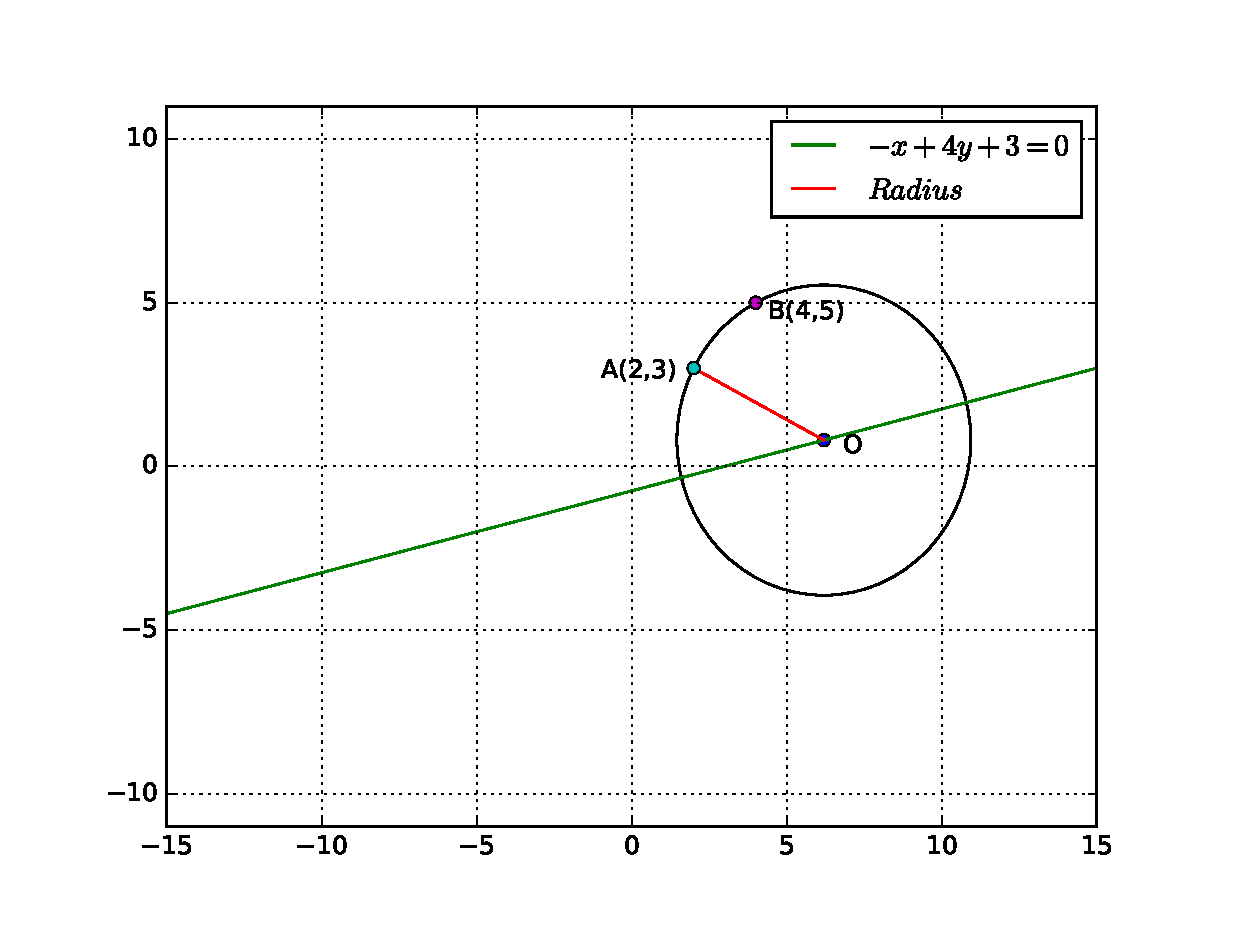
\includegraphics[width = 0.9\textwidth]{./Plot.eps}
  		\end{figure}
	}
\end{document}